\section{Introducci\'on}
La competencia de Seaperch es un evento organizado por la guardia naval de Estados Unidos, con el fin
de promover en los estudiantes el inter\'es por carreras de STEM (Science, Technology, Engineering and Mathematics).
Lo logra a trav\'es del reto acu\'atico que consiste en la construcci\'on de un submarino y la superaci\'on de obst\'aculos.

\section{Objetivos}
\begin{itemize}
 \item Dise\~nar en un software de CAD el modelo de un submarino Seaperch
 \item Fabricar un submarino Seaperch
 \item Dise\~nar y construir el sistema de control del submarino
\end{itemize}

\section{Descripci\'on y Presentaci\'on}
El desarrollo del proyecto se llev\'o a cabo en tres etapas:
\begin{itemize}
 \item Dise\~no virtual
 \item Prototipo
 \item Producto finals
\end{itemize}

\section{Dise\~no Asistido por Computadora}
Para el dise\~no en CAD, se realizaron dos versiones del submarino: una en Siemens NX 10 y otra en FreeCAD 0.17.
El modelo en FreeCAD se elabor\'o durante el fin de semana, por lo que su disponibilidad permiti\'o dise\~nar y construir
la estructura del submarino durante un \'unico fin de semana. En la figura 1 se muestra la vista isom\'etrica del
submarino en FreeCAD.\\

Asimismo, se utiliz\'o FreeCAD para dise\~nar los contenedores de los motores, y el ap\'endice que mover\'ia los aros del reto.
Los contenedores se fabricaron mediante impresi\'on 3D de PLA en colores azul y transparente. Se contrataron dos proveedores
para reducir el tiempo de espera para obtener todas las impresiones necesarias. La figura 2 muestra la vista
isom\'etrica del contenedor de los motores.\\

 \begin{figure}[!htbp]
 \centering
 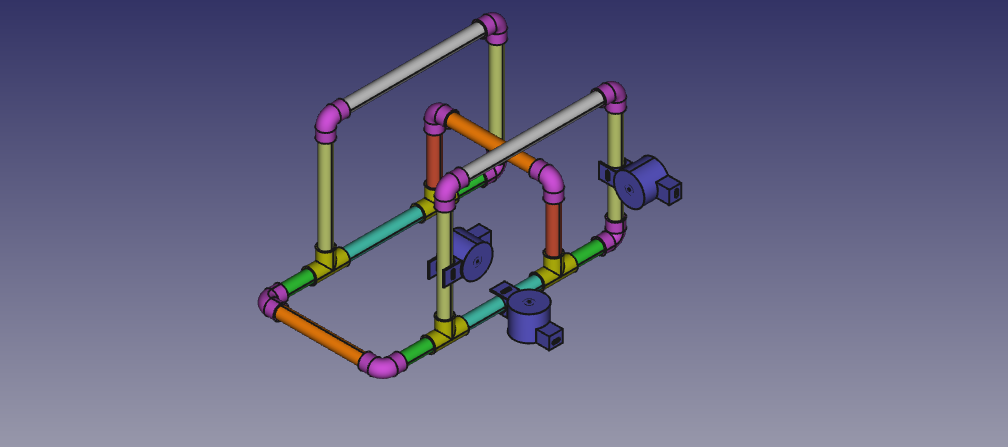
\includegraphics [scale=0.5]
  {./img/seaperch_freecad.png}
  \caption{Modelo en FreeCAD}
 \end{figure}

 \begin{figure}[!htbp]
 \centering
 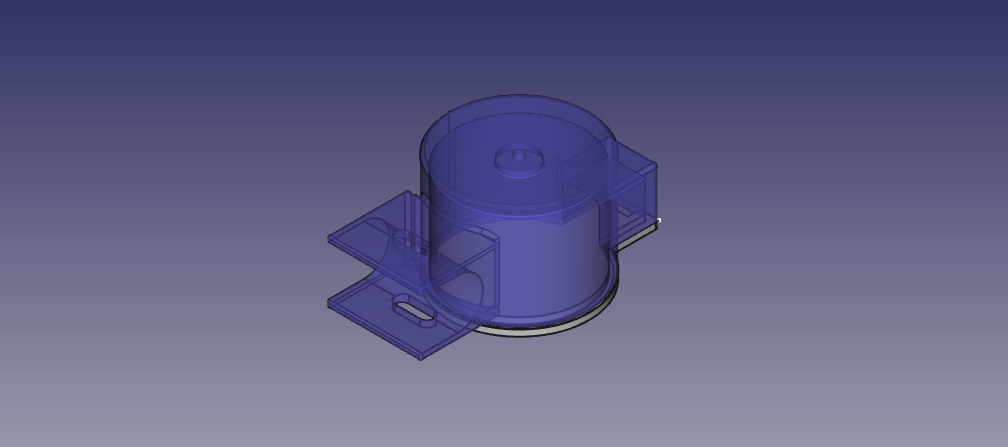
\includegraphics [scale=0.5]
  {./img/seaperch_motor.png}
  \caption{Modelo en FreeCAD}
 \end{figure}

Se utiliz\'o NX para generar un render de alta calidad del modelo, generar el layout del submarino y las proyecciones del mismo
para su posible armado. En las figuras 3, 4, y 5 se muestran los resultados.

 \begin{figure}[!htbp]
 \centering
 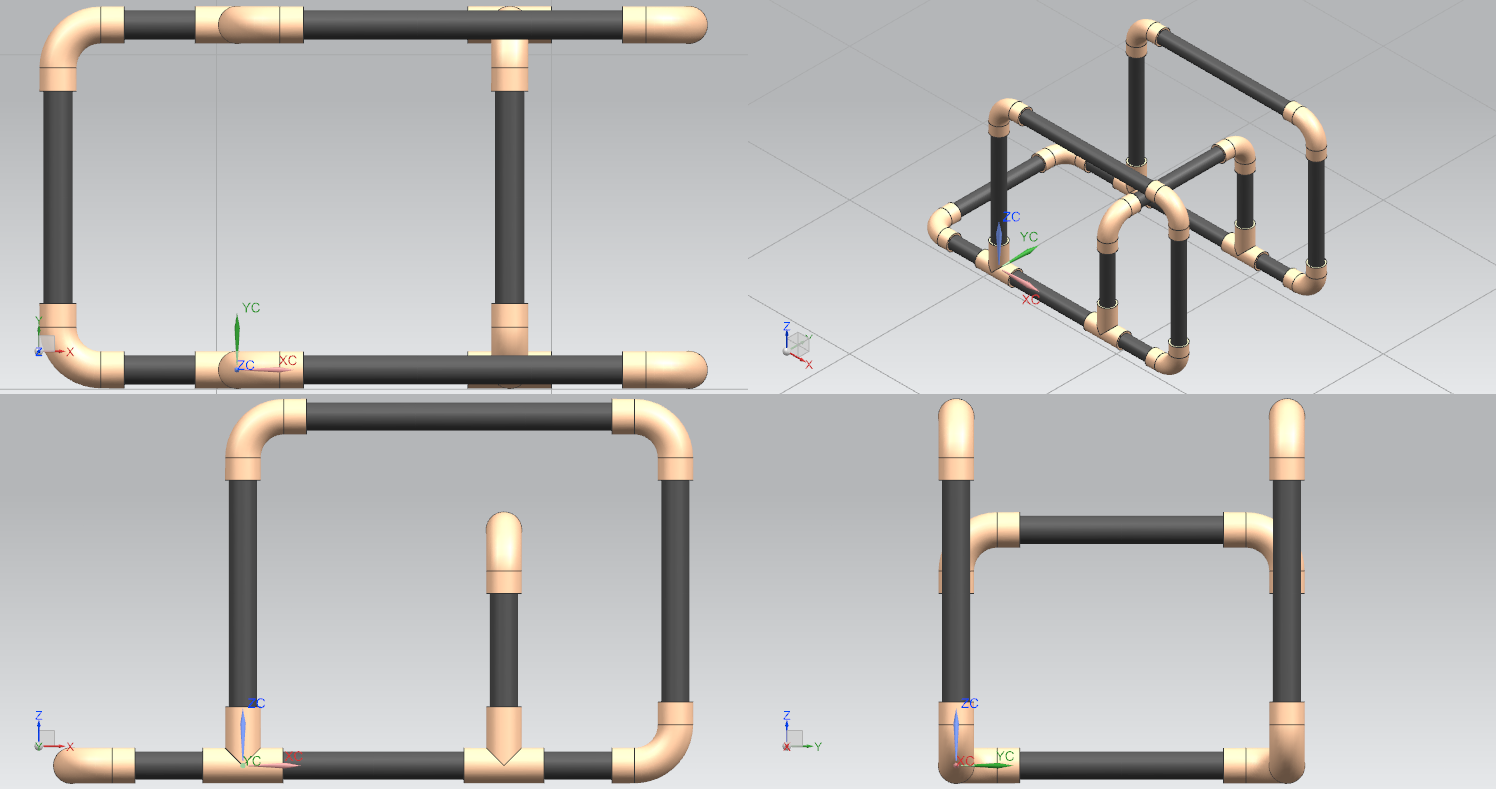
\includegraphics [scale=0.25]
  {./img/seaperch_nx.png}
  \caption{Modelo en NX}
 \end{figure}

  \begin{figure}[!htbp]
 \centering
 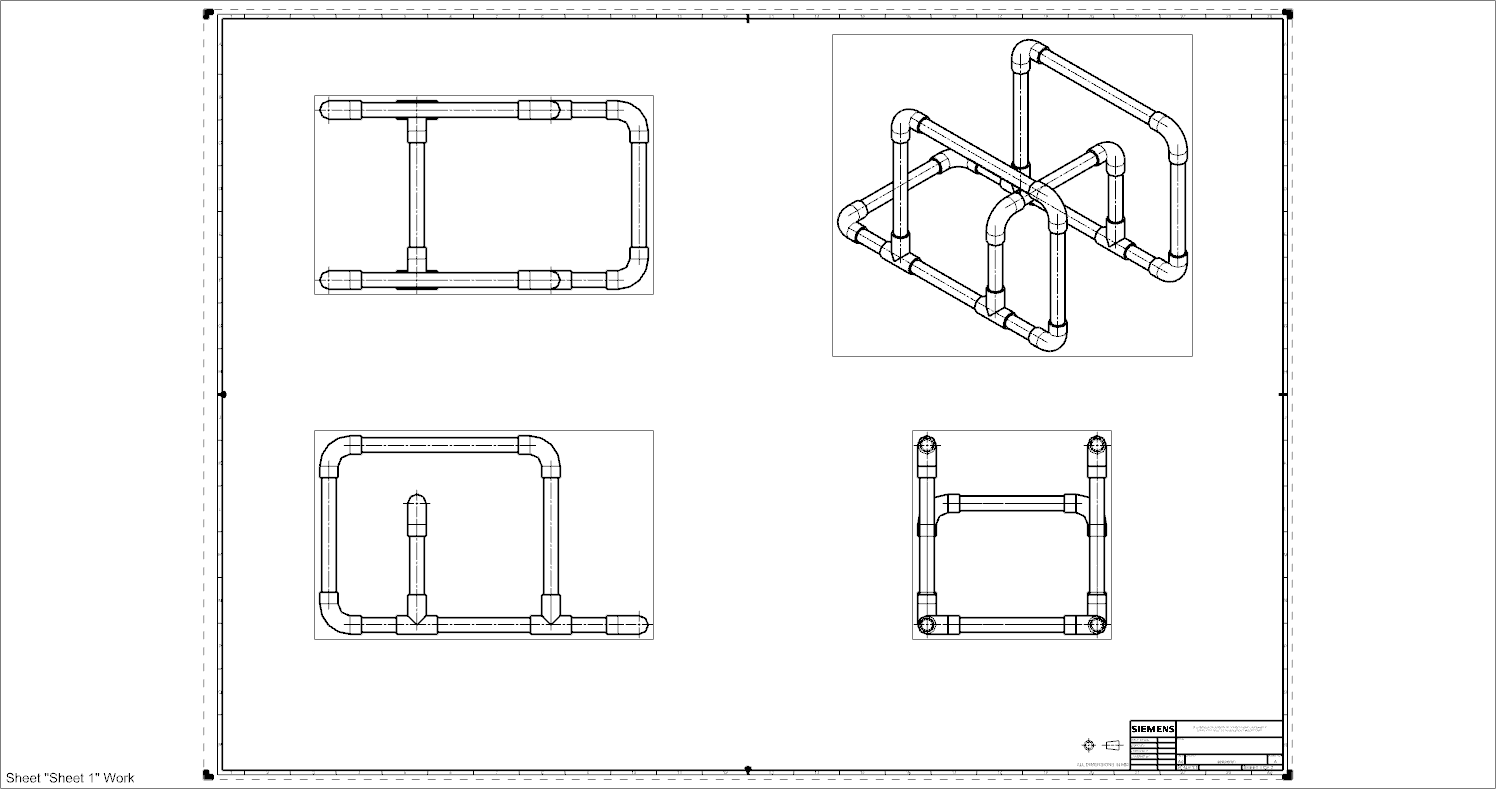
\includegraphics [scale=0.25]
  {./img/seaperch_vistas.png}
  \caption{Proyecciones del modelo}
 \end{figure}

  \begin{figure}[!htbp]
 \centering
 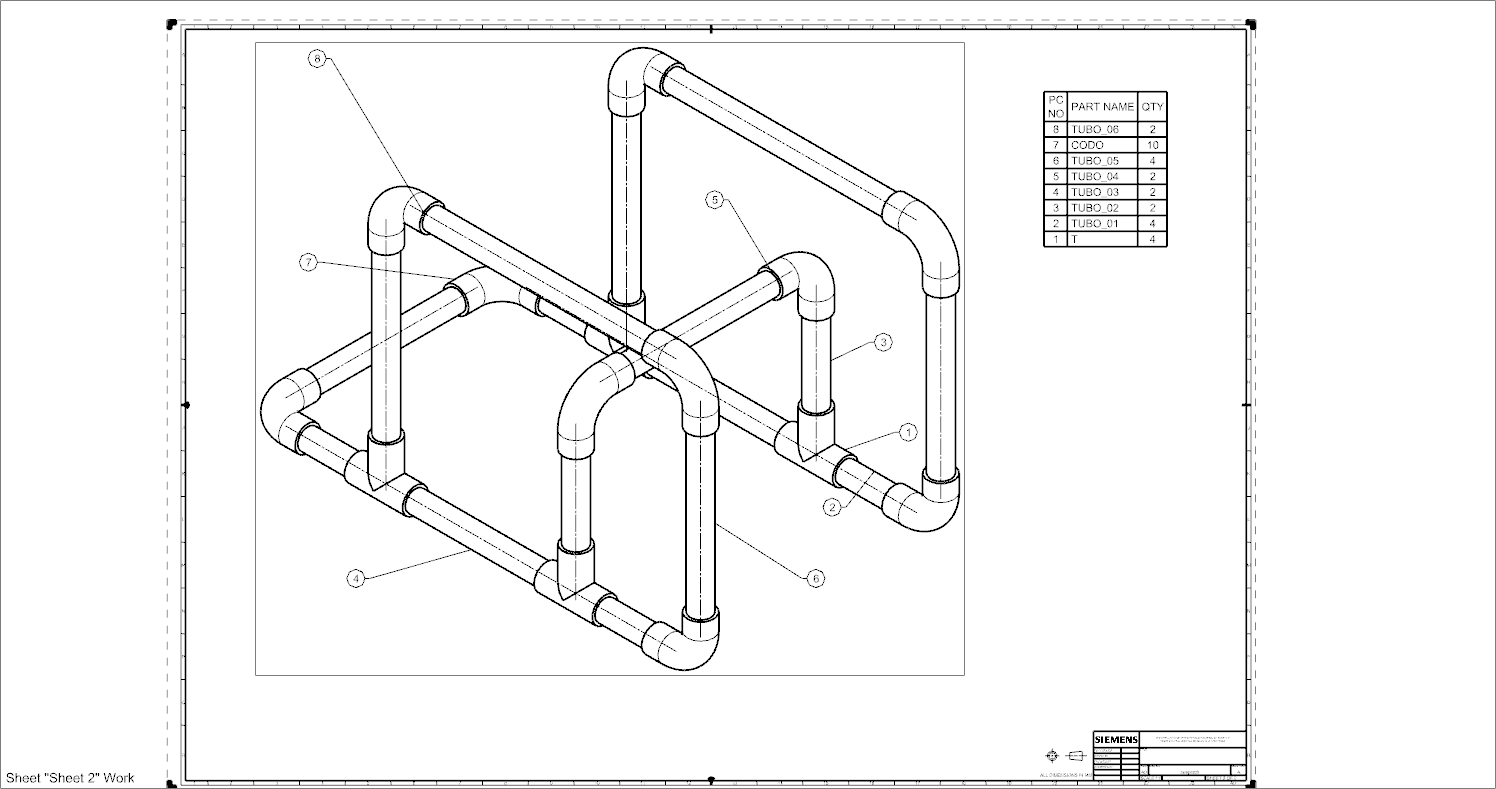
\includegraphics [scale=0.25]
  {./img/seaperch_piezas.png}
  \caption{Distribuci\'on de piezas}
 \end{figure}

 \pagebreak

\section{Electr\'onica}
Se utiliz\'o Proteus para dise\~nar el circuito electr\'onico para controlar el submarino. Se opt\'o por utlizar
un microcontrolador como el coraz\'on del sistema de control. El PIC 16F877, posee una presentaci\'on insertable
en protoboards de 40 pines, la cual facilita su uso en prototipos y una programaci\'on r\'apida con hardware disponible
en la escuela.

Se dise\~n\'o una PCB de 10 cm de alto por 15 cm de largo para contener todo el sistema de control. Se emple\'o la
t\'ecnica de transferencia por acetato para asegurarse que las pistas se fijaran en la placa de cobre. La placa de cobre se
trat\'o previamente para remover suciedad y grasa que se encontraba en su superficie.


\section{Programaci\'on}
Se hizo uso de la suite de programaci\'on de Mikrobasic para dise\~nar y compilar el c\'odigo que se program\'o en el PIC.
Para cargar el c\'odigo en el PIC se hizo uso de un PIC Kit 2 de Microchip.